% Options for packages loaded elsewhere
\PassOptionsToPackage{unicode}{hyperref}
\PassOptionsToPackage{hyphens}{url}
\PassOptionsToPackage{dvipsnames,svgnames,x11names}{xcolor}
%
\documentclass[
  letterpaper,
  DIV=11,
  numbers=noendperiod]{scrreprt}

\usepackage{amsmath,amssymb}
\usepackage{iftex}
\ifPDFTeX
  \usepackage[T1]{fontenc}
  \usepackage[utf8]{inputenc}
  \usepackage{textcomp} % provide euro and other symbols
\else % if luatex or xetex
  \usepackage{unicode-math}
  \defaultfontfeatures{Scale=MatchLowercase}
  \defaultfontfeatures[\rmfamily]{Ligatures=TeX,Scale=1}
\fi
\usepackage{lmodern}
\ifPDFTeX\else  
    % xetex/luatex font selection
\fi
% Use upquote if available, for straight quotes in verbatim environments
\IfFileExists{upquote.sty}{\usepackage{upquote}}{}
\IfFileExists{microtype.sty}{% use microtype if available
  \usepackage[]{microtype}
  \UseMicrotypeSet[protrusion]{basicmath} % disable protrusion for tt fonts
}{}
\makeatletter
\@ifundefined{KOMAClassName}{% if non-KOMA class
  \IfFileExists{parskip.sty}{%
    \usepackage{parskip}
  }{% else
    \setlength{\parindent}{0pt}
    \setlength{\parskip}{6pt plus 2pt minus 1pt}}
}{% if KOMA class
  \KOMAoptions{parskip=half}}
\makeatother
\usepackage{xcolor}
\setlength{\emergencystretch}{3em} % prevent overfull lines
\setcounter{secnumdepth}{5}
% Make \paragraph and \subparagraph free-standing
\ifx\paragraph\undefined\else
  \let\oldparagraph\paragraph
  \renewcommand{\paragraph}[1]{\oldparagraph{#1}\mbox{}}
\fi
\ifx\subparagraph\undefined\else
  \let\oldsubparagraph\subparagraph
  \renewcommand{\subparagraph}[1]{\oldsubparagraph{#1}\mbox{}}
\fi


\providecommand{\tightlist}{%
  \setlength{\itemsep}{0pt}\setlength{\parskip}{0pt}}\usepackage{longtable,booktabs,array}
\usepackage{calc} % for calculating minipage widths
% Correct order of tables after \paragraph or \subparagraph
\usepackage{etoolbox}
\makeatletter
\patchcmd\longtable{\par}{\if@noskipsec\mbox{}\fi\par}{}{}
\makeatother
% Allow footnotes in longtable head/foot
\IfFileExists{footnotehyper.sty}{\usepackage{footnotehyper}}{\usepackage{footnote}}
\makesavenoteenv{longtable}
\usepackage{graphicx}
\makeatletter
\def\maxwidth{\ifdim\Gin@nat@width>\linewidth\linewidth\else\Gin@nat@width\fi}
\def\maxheight{\ifdim\Gin@nat@height>\textheight\textheight\else\Gin@nat@height\fi}
\makeatother
% Scale images if necessary, so that they will not overflow the page
% margins by default, and it is still possible to overwrite the defaults
% using explicit options in \includegraphics[width, height, ...]{}
\setkeys{Gin}{width=\maxwidth,height=\maxheight,keepaspectratio}
% Set default figure placement to htbp
\makeatletter
\def\fps@figure{htbp}
\makeatother

\KOMAoption{captions}{tableheading}
\makeatletter
\@ifpackageloaded{tcolorbox}{}{\usepackage[skins,breakable]{tcolorbox}}
\@ifpackageloaded{fontawesome5}{}{\usepackage{fontawesome5}}
\definecolor{quarto-callout-color}{HTML}{909090}
\definecolor{quarto-callout-note-color}{HTML}{0758E5}
\definecolor{quarto-callout-important-color}{HTML}{CC1914}
\definecolor{quarto-callout-warning-color}{HTML}{EB9113}
\definecolor{quarto-callout-tip-color}{HTML}{00A047}
\definecolor{quarto-callout-caution-color}{HTML}{FC5300}
\definecolor{quarto-callout-color-frame}{HTML}{acacac}
\definecolor{quarto-callout-note-color-frame}{HTML}{4582ec}
\definecolor{quarto-callout-important-color-frame}{HTML}{d9534f}
\definecolor{quarto-callout-warning-color-frame}{HTML}{f0ad4e}
\definecolor{quarto-callout-tip-color-frame}{HTML}{02b875}
\definecolor{quarto-callout-caution-color-frame}{HTML}{fd7e14}
\makeatother
\makeatletter
\@ifpackageloaded{bookmark}{}{\usepackage{bookmark}}
\makeatother
\makeatletter
\@ifpackageloaded{caption}{}{\usepackage{caption}}
\AtBeginDocument{%
\ifdefined\contentsname
  \renewcommand*\contentsname{Índice}
\else
  \newcommand\contentsname{Índice}
\fi
\ifdefined\listfigurename
  \renewcommand*\listfigurename{Lista de Figuras}
\else
  \newcommand\listfigurename{Lista de Figuras}
\fi
\ifdefined\listtablename
  \renewcommand*\listtablename{Lista de Tabelas}
\else
  \newcommand\listtablename{Lista de Tabelas}
\fi
\ifdefined\figurename
  \renewcommand*\figurename{Figura}
\else
  \newcommand\figurename{Figura}
\fi
\ifdefined\tablename
  \renewcommand*\tablename{Tabela}
\else
  \newcommand\tablename{Tabela}
\fi
}
\@ifpackageloaded{float}{}{\usepackage{float}}
\floatstyle{ruled}
\@ifundefined{c@chapter}{\newfloat{codelisting}{h}{lop}}{\newfloat{codelisting}{h}{lop}[chapter]}
\floatname{codelisting}{Listagem}
\newcommand*\listoflistings{\listof{codelisting}{Lista de Listagens}}
\makeatother
\makeatletter
\makeatother
\makeatletter
\@ifpackageloaded{caption}{}{\usepackage{caption}}
\@ifpackageloaded{subcaption}{}{\usepackage{subcaption}}
\makeatother
\ifLuaTeX
\usepackage[bidi=basic]{babel}
\else
\usepackage[bidi=default]{babel}
\fi
\babelprovide[main,import]{portuguese}
% get rid of language-specific shorthands (see #6817):
\let\LanguageShortHands\languageshorthands
\def\languageshorthands#1{}
\ifLuaTeX
  \usepackage{selnolig}  % disable illegal ligatures
\fi
\usepackage{bookmark}

\IfFileExists{xurl.sty}{\usepackage{xurl}}{} % add URL line breaks if available
\urlstyle{same} % disable monospaced font for URLs
\hypersetup{
  pdftitle={R e RStudio para Iniciantes},
  pdfauthor={GPEQ/UFRJ},
  pdflang={pt},
  colorlinks=true,
  linkcolor={blue},
  filecolor={Maroon},
  citecolor={Blue},
  urlcolor={Blue},
  pdfcreator={LaTeX via pandoc}}

\title{R e RStudio para Iniciantes}
\usepackage{etoolbox}
\makeatletter
\providecommand{\subtitle}[1]{% add subtitle to \maketitle
  \apptocmd{\@title}{\par {\large #1 \par}}{}{}
}
\makeatother
\subtitle{Material de Apoio para Cursos Quantitativos do Instituto de
Economia da Universidade Federal do Rio de Janeiro (IE/UFRJ)}
\author{GPEQ/UFRJ}
\date{2024-03-26}

\begin{document}
\maketitle

\renewcommand*\contentsname{Índice}
{
\hypersetup{linkcolor=}
\setcounter{tocdepth}{2}
\tableofcontents
}
\bookmarksetup{startatroot}

\chapter*{Prefácio}\label{sec-preface}
\addcontentsline{toc}{chapter}{Prefácio}

\markboth{Prefácio}{Prefácio}

\section*{O que você vai aprender}\label{o-que-vocuxea-vai-aprender}
\addcontentsline{toc}{section}{O que você vai aprender}

\markright{O que você vai aprender}

Pretendemos que você domine o \emph{mínimo} necessário de programação em
R para executar as tarefas que podem ser requisitadas pelo seu
professor, independentemente do curso da área quantitativa em que
estiver. Em outras palavras, se te pedirem algo que deva ser elaborado
com auxílio de programação em R, você será capaz de fazê-lo após ler
este material\footnote{Esperamos que os empecilhos que apareçam não
  sejam por conta de alguma dificuldade no ato de programar em si, mas
  por dúvidas com relação à matéria propriamente dita. De qualquer
  forma, fique tranquilo: se você não entendeu alguma parte do material,
  estaremos \textbf{sempre} abertos a te ajudar!}.

Na prática, o quê significa \emph{dominar o mínimo necessário de
programação em R?} Inclui entender alguns \emph{conceitos} básicos --
para quê serve a programação em nosso contexto, o que é a linguagem de
programação R, o que é o RStudio, entre outros -- assim como a
\emph{sintaxe} da linguagem -- ou seja, o ato de escrever um código
interpretável propriamente dito.

\section*{\texorpdfstring{O que você \textbf{não} vai
aprender}{O que você não vai aprender}}\label{o-que-vocuxea-nuxe3o-vai-aprender}
\addcontentsline{toc}{section}{O que você \textbf{não} vai aprender}

\markright{O que você \textbf{não} vai aprender}

Não estamos em um curso de Ciência da Computação: você não irá aprender
terminologias difíceis e/ou como a programação, de modo geral, funciona
nos \emph{detalhes}. Em outras palavras, vamos nos concentrar apenas em
entender o necessário para construir e executar \emph{códigos} em R (não
se preocupe, ainda explicaremos o que é um \emph{código em R}) a partir
das tarefas que seu professor poderá pedir.

Além disso, o material não te dará proficiência em R. O que queremos
dizer com isso? Bom, queremos dizer que você não será uma pessoa que
dominará o R de forma \emph{avançada}. Novamente: aqui, te ensinaremos
apenas o necessário para que consiga concluir os cursos da área
quantitativa. Mas, se você realmente quiser alcançar níveis mais altos,
alguns livros podem te ajudar:

\begin{itemize}
\item
  \href{https://r4ds.hadley.nz/}{R for Data Science (2ª edição)}
\item
  \href{https://livro.curso-r.com/index.html}{Ciência de Dados em R}
\item
  \href{https://bookdown.org/hneth/ds4psy/}{Data Science for
  Psychologists}
\item
  \href{https://bookdown.org/rwnahhas/IntroToR/}{An Introduction to R
  for Research}
\end{itemize}

\section*{Preciso saber alguma coisa de forma
antecipada?}\label{preciso-saber-alguma-coisa-de-forma-antecipada}
\addcontentsline{toc}{section}{Preciso saber alguma coisa de forma
antecipada?}

\markright{Preciso saber alguma coisa de forma antecipada?}

\textbf{Não}. Você não precisa saber absolutamente \emph{nada} de
programação em R -- não precisa nem mesmo saber o que o termo
\emph{programação} significa. O intuito do material é justamente te
introduzir aos conceitos mais básicos!

\textbf{A única coisa que você precisará será de acesso à um computador
com internet}. Utilizar um computador é necessário pois é nele onde
ocorre o ato de programar; ter internet é importante porquê, ao longo
dos captíulos, precisaremos que você realize o \emph{download} de certos
arquivos -- seja para instalar o R e o RStudio ou para \emph{importar}
algum arquivo diretamente para este último (não se preocupe, ainda
explicaremos o que \emph{importação} de um arquivo significa).

\section*{Como o material está
organizado}\label{como-o-material-estuxe1-organizado}
\addcontentsline{toc}{section}{Como o material está organizado}

\markright{Como o material está organizado}

O material está organizado em sete capítulos: o primeiro, que te mostra
a motivação para programar, além de outros seis que buscam, em primeiro
lugar, te guiar na instalação do R e RStudio e, na sequência, ensinar
comandos e conceitos básicos que serão necessários ao longo dos cursos.
Com intuito de facilitar o aprendizado, cada capítulo foi repartido em
um certo número de seções (e subseções, quando necessário).

A lista de capítulos pode ser observada no menu à \emph{esquerda}. Por
sua vez, a lista de seções do capítulo em que você estiver pode ser
observada no menu à \emph{direita}. Perceba que, para ser direcionado a
um determinado capítulo/seção, basta clicar em seu nome.

\begin{center}
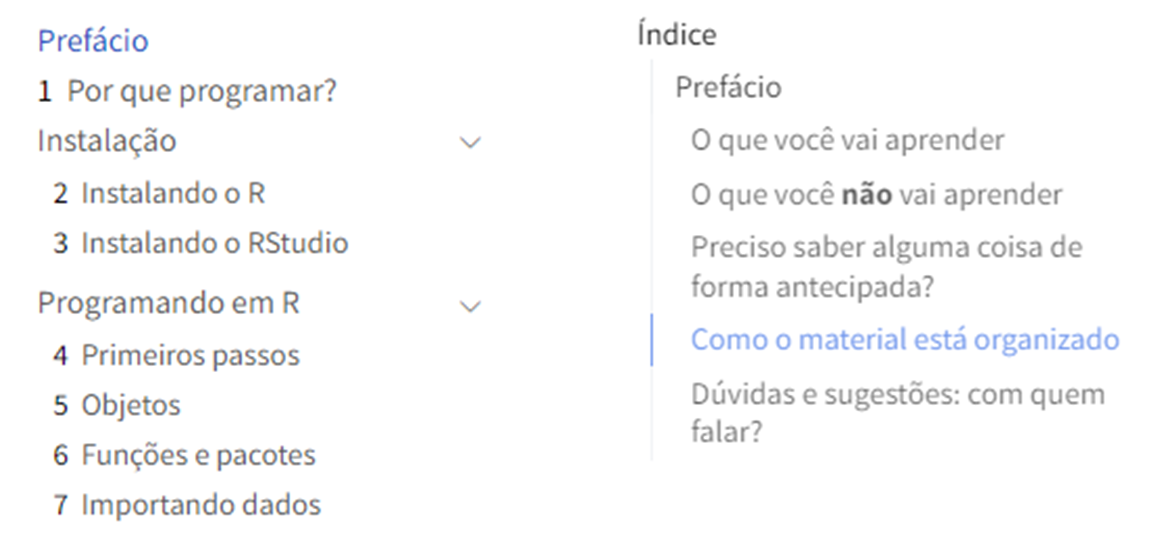
\includegraphics[width=5.63542in,height=\textheight]{images/clipboard-250739170.png}
\end{center}

\emph{``Caramba, queria tanto acessar uma parte específica do material
que não lembro muito bem onde está\ldots{} E agora?''} Sem problemas:
você pode pesquisar partes do texto ou palavras-chave no campo em branco
logo acima do Prefácio!

\begin{center}

\includegraphics[width=2.71875in,height=\textheight]{images/clipboard-2391069838.png}
\end{center}

\section*{Dúvidas e sugestões: com quem
falar?}\label{duxfavidas-e-sugestuxf5es-com-quem-falar}
\addcontentsline{toc}{section}{Dúvidas e sugestões: com quem falar?}

\markright{Dúvidas e sugestões: com quem falar?}

\emph{``Ué, no meu computador não aparece isso!''\\
``Caramba, achei aquele trechinho ali meio confuso\ldots{} podia
melhorar\ldots{}''\\
``Nossa, que material show!''}

Surgiu alguma dúvida ou então quer dar alguma sugestão de melhoria?
Estamos totalmente abertos à qualquer tipo de crítica! Envie uma
mensagem para \url{pedro.hemsley@ie.ufrj.br}.

\bookmarksetup{startatroot}

\chapter{Por que programar?}\label{sec-intro}

De forma simplificada, é possível definir o ato de programar como a
passagem de determinados comandos para o computador, com a finalidade de
que ele execute determinada tarefa. Se você deseja algo que pode ser
feito de forma mais eficiente por uma máquina, provavelmente escreverá
um código que seja interpretável por esta, de modo que seu desejo se
concretize.

A capacidade de programar tornou-se uma habilidade essencial,
especialmente para aqueles que desejam explorar o mundo da estatística e
da matemática aplicados à determinada ciência social. Por exemplo, no
contexto de interseção entre economia e matemática -- principalmente na
elaboração e solução de modelos teóricos -- e entre economia e
estatística -- testando hipóteses e realizando previsões -- a
programação se coloca como uma ferramenta muito útil para economizar
tempo de cálculo e garantir que, caso necessário, o mesmo processo seja
concluído múltiplas vezes sem erros. Em outras palavras, a programação
aplicada à determinada ciência social, como a economia, traz duas
principais vantagens, exploradas melhoras a seguir.

\section{Redução no tempo de
cálculo}\label{reduuxe7uxe3o-no-tempo-de-cuxe1lculo}

A primeira vantagem é a redução no tempo de cálculo de certos
procedimentos que, se feitos de forma manual, levariam vários minutos,
horas ou até mesmo dias. Vamos deixar mais claro com um exemplo.

No ensino fundamental, você aprendeu a resolver um sistema de equações
simultâneas com 2 variáveis e 2 equações, muito provavelmente pelo
método de substituição. Não levava muito tempo, certo? Acontece que, na
cadeira de Álgebra Linear, você aprenderá como solucionar sistemas de
\(n\) equações e \(n\) variáveis. Normalmente, quanto maior \(n\), maior
será a dificuldade de encontrar a solução do sistema. Ainda que existam
\emph{algoritmos} que permitam encontrar a solução de forma mais rápida,
certo tempo será perdido se você os replicar de forma \emph{manual}.

Com auxílio da programação, no entanto, é possível implementar estes
mesmos algoritmos para obter o resultado de forma quase que
\emph{instantânea.} \emph{O tempo que você levaria fazendo o
procedimento manual praticamente se reduz a zero -- ou fica mínimo, em
relação ao incial.} Observe que você ainda deve focar em saber como o
algoritmo funciona, do contrário não será capaz de julgar se o que a
máquina fez é realmente aquilo que você desejava.

\section{Automação de processos}\label{automauxe7uxe3o-de-processos}

Na seção anterior, repare que estavamos discorrendo implicitamente sobre
cálculos de ocorrência única -- ou seja, realizamos o cálculo uma vez e
não teríamos mais interesse de fazê-lo novamente em um futuro próximo.
No entanto, outro benefício prático do ato de programar é a automação de
tarefas repetitivas. Com a programação, é possível escrever e salvar
\emph{scripts} que automatizam tarefas tediosas de manipulação e análise
de dados, permitindo que os pesquisadores se concentrem em questões
analíticas de maior relevância.

Por exemplo, imagine que alguém te peça para calcular a média de certos
valores que mudam de dia para dia. Você pode facilmente elaborar um
\emph{scipt} que, a partir de determinados números (sem especificar
quais são), calcule sua média. Uma vez escrito e salvo, você pode passar
a executá-lo sempre que quiser -- no exemplo, todos os dias.

\section{Vamos programar!}\label{vamos-programar}

Em suma, aprender a programar oferece uma série de vantagens tangíveis
para quem trabalha com estatística e matemática. Ela tornar o trabalho
mais eficiente e produtivo, permitindo que os profissionais explorem
dados de maneiras antes inimagináveis e desenvolvam soluções
personalizadas para os desafios enfrentados em suas áreas de atuação.

No restante do material, aprenderemos a programar utilizando a
\emph{linguagem de programação R.} Em outras palavras, aprenderemos sua
\emph{sintaxe}, isto é, a forma de escrever comandos corretamente para
que a máquina seja capaz de interpretar e executar o que queremos como
resultado.

\bookmarksetup{startatroot}

\chapter{Instalando o R}\label{instalando-o-r}

Nesse capítulo, iremos aprender como baixar e instalar o R para
Windows\footnote{Você pode realizar procedimento equivalente para
  sistemas operacionais Linux, apenas alterando a opção de
  \emph{download} quando necessário -- isto é, selecionando as opções em
  que esteja escrito `Linux', ao invés de `Windows'.}! Optamos por
dividir o passo a passo em 7 etapas -- mas fique tranquilo, não são
passos grandes, apenas fizemos dessa forma para que o conteúdo fique bem
\emph{mastigado}, fácil de entender.

\begin{tcolorbox}[enhanced jigsaw, opacityback=0, breakable, leftrule=.75mm, toprule=.15mm, colbacktitle=quarto-callout-tip-color!10!white, toptitle=1mm, colback=white, left=2mm, title=\textcolor{quarto-callout-tip-color}{\faLightbulb}\hspace{0.5em}{Alguns conceitos iniciais (Opcional)}, bottomtitle=1mm, titlerule=0mm, arc=.35mm, rightrule=.15mm, bottomrule=.15mm, opacitybacktitle=0.6, coltitle=black, colframe=quarto-callout-tip-color-frame]

Antes de começar, vamos entender alguns conceitos. A ideia aqui é te
ensinar o que significam algumas nomenclaturas e siglas que aparecem ao
longo do processo de instalação, em especial \emph{R Foundation} e
\emph{CRAN}. Essa parte é totalmente \emph{opcional} e você pode pular
direto para o passo a passo caso esteja sem tempo -- ou até mesmo
interesse.

\begin{itemize}
\item
  \textbf{R Foundation}: é uma empresa sem fins lucrativos, criada pelos
  principais desenvolvedores da linguagem. Quais são seus objetivos?
  Basicamente três: (i) administrar os direitos autorais da linguagem --
  e, por consequência, manter seu uso como livre; (ii) apoiar o
  desenvolvimento do R como um todo, isto é, fornecer informações e
  criar novos usos básicos, elaborar conferências, guias, entre outros;
  (iii) servir como ponto focal para todos os usuários da linguagem que
  desejem interagir com a comunidade de desenvolvedores. De forma
  resumida, a R Foundation é como se fosse a instituição provedora do
  básico da linguagem, que busca sempre atualizar e mantê-lo de pé. Se
  você instala o R e, logo em seguida, percebe que alguma de suas
  atribuições não está em perfeito funcionamento, provavelmente terá que
  comunicar à essas pessoas. Grosso modo, exerce um papel próximo ao da
  Microsoft com o Excel, por exemplo. Uma observação (importante): como
  o R é um software livre, qualquer pessoa pode desenvolver novas
  funções ou recursos a partir da linguagem. Por esse motivo, para
  recursos que estejam além da \emph{base do R}, você deve recorrer à
  quem os criou! Por exemplo, com relação ao RStudio (que conheceremos
  mais à frente), devemos nos reportar à empresa Posit, sua
  desenvolvedora. Na prática, raramente (para não dizer nunca) iremos
  reportar alguma coisa à R Foundation, mas sim aos desenvolvedores
  daquele pacote/extensão específico (fique tranquilo, explicaremos mais
  à frente o conceito de \emph{pacote} para a linguagem).
\item
  \textbf{CRAN} (Comprehensive R Archive Network): segundo o própio, é
  ``\emph{uma coleção de sites que carrega material idêntico,
  consistindo nas distribuições do R, extensões contriubídas,
  documentação e arquivos binários de R}''. \emph{`Meu Deus, o que isso
  significa?'} Simples: apenas uma coleção de endereços da internet em
  que podemos baixar a versão mais recente do R, assim como pacotes.
  Quem mantém o CRAN? Instituições voluntárias; em seus sites, a parte
  onde é possível baixar arquivos relacionados ao R é chamada de
  \emph{mirror}. E com quais recursos o CRAN se mantém? Com os da
  própria instituição participante (principalmente em termos de
  colaboradores) e, também, da R Foundation!
\end{itemize}

Essa história toda para dizer: \textbf{o arquivo básico que iremos
baixar para instalar o R será obtido através de algum \emph{mirror} do
CRAN, isto é, a parte do site de alguma instituição voluntária em
colaboração com a R Foundation.}

\end{tcolorbox}

\section{Sete passos}\label{sete-passos}

\begin{enumerate}
\def\labelenumi{\arabic{enumi}.}
\item
  O primeiro passo consiste em escolher um repositório (\emph{mirror)}
  para baixar o R. No endereço
  \url{https://cran.r-project.org/mirrors.html} encontramos todas as
  opções disponíveis, por país e em ordem alfabética. No seu computador,
  deverá aparecer a seguinte tela:

  \begin{center}
  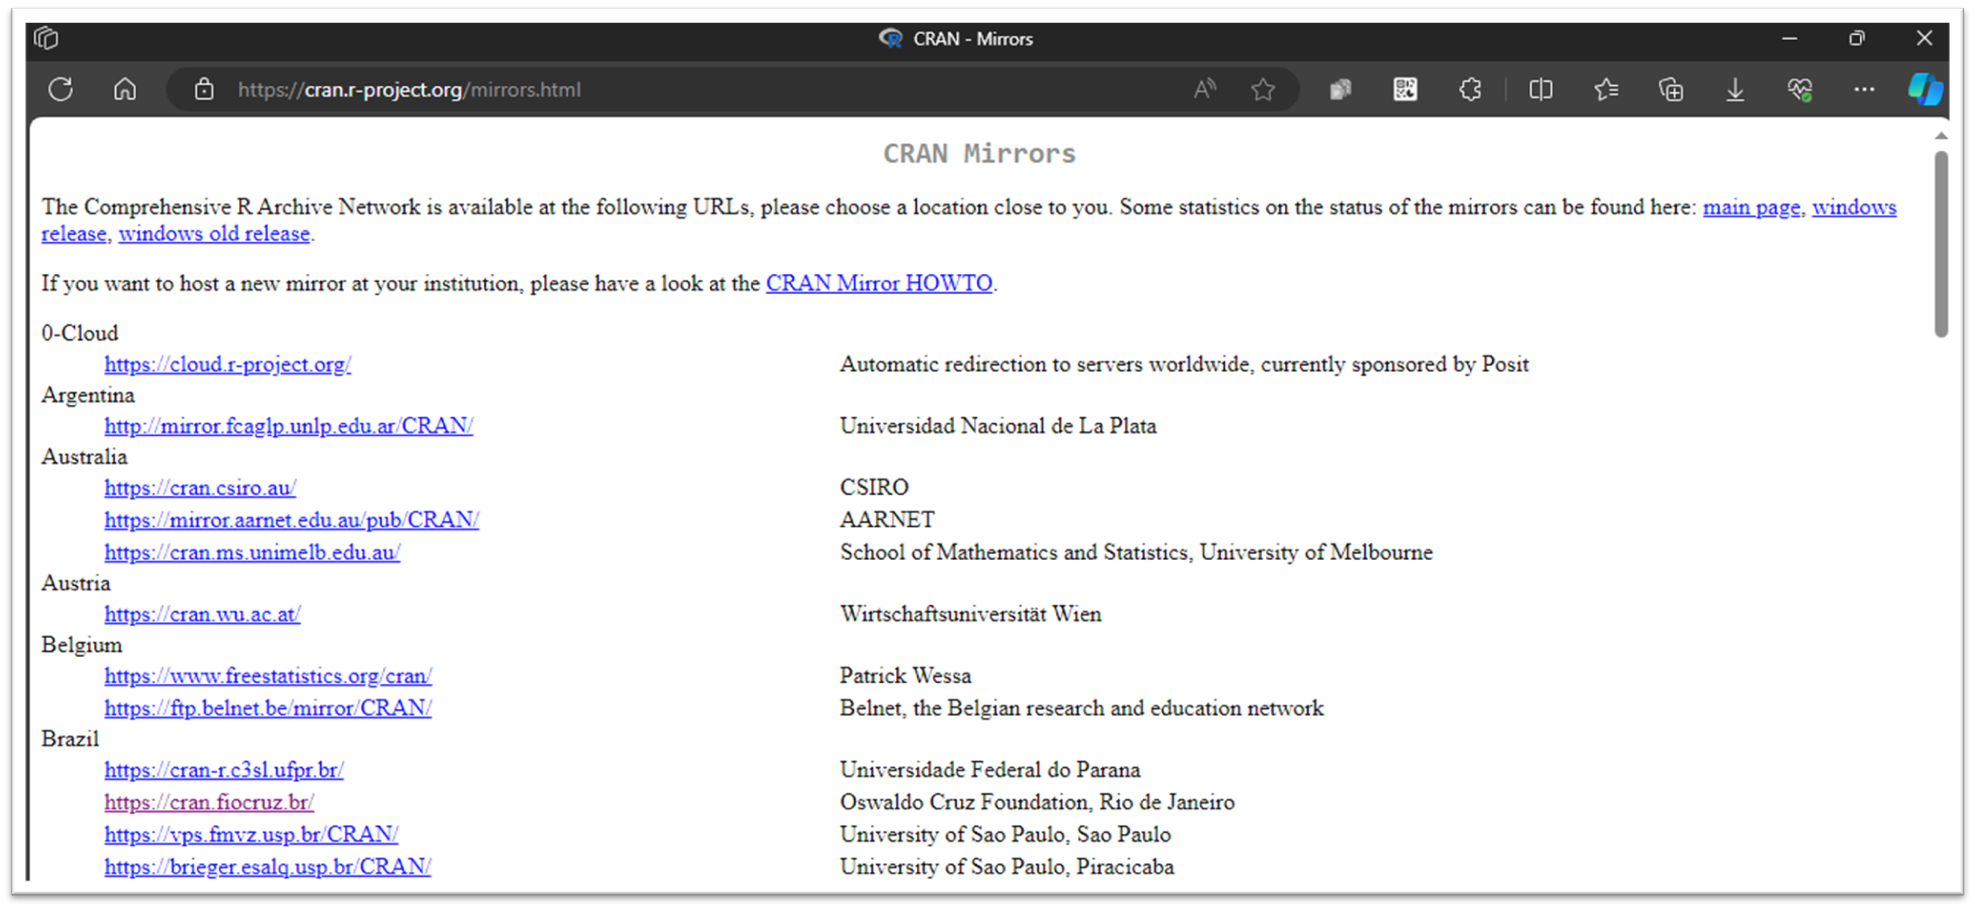
\includegraphics{images/clipboard-3074288328.png}
  \end{center}
\item
  Por questões de rapidez/latência, o ideal é escolher o repositório
  mais próximo de você. Considerando que todos estejam no Rio de
  Janeiro, vamos então utilizar o \emph{mirror} da Fiocruz.

  \begin{center}
  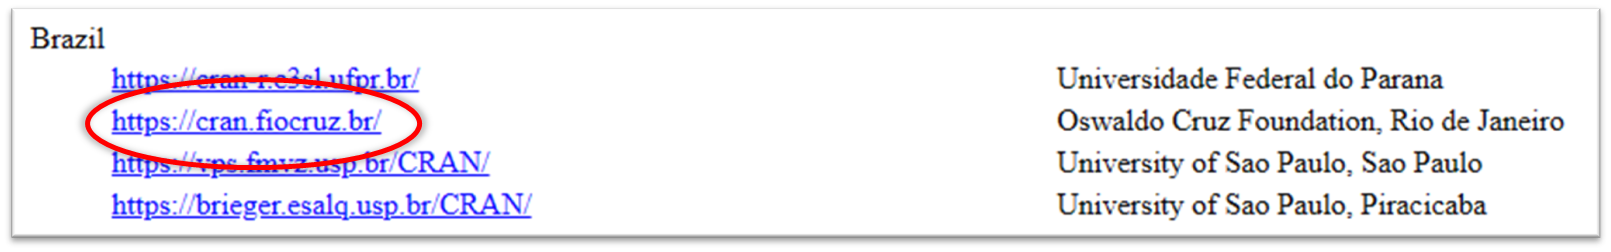
\includegraphics{images/clipboard-283220567.png}
  \end{center}
\item
  Como essa apostila foca na instalação para sistemas operacionais do
  tipo Windows, vamos clicar então em \emph{Download R for Windows}, na
  parte superior da página.

  \begin{center}
  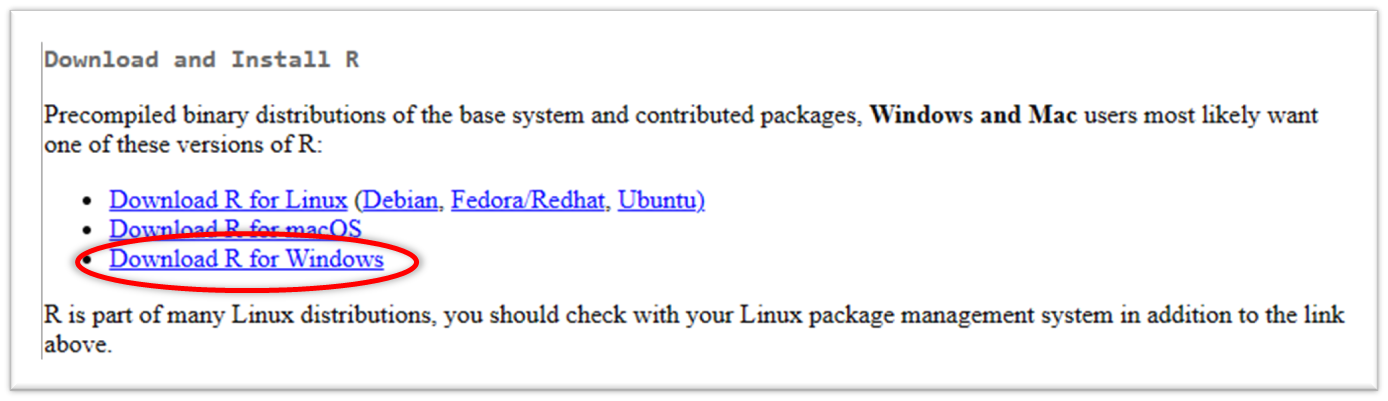
\includegraphics{images/clipboard-1477947543.png}
  \end{center}
\item
  Na página seguinte, clique em `base'. Grosso modo, como o nome já
  indica, iremos baixar os aquivos \emph{base} do R -- ou seja, o mínimo
  necessário que você precisará para poder executar algum código.

  \begin{center}
  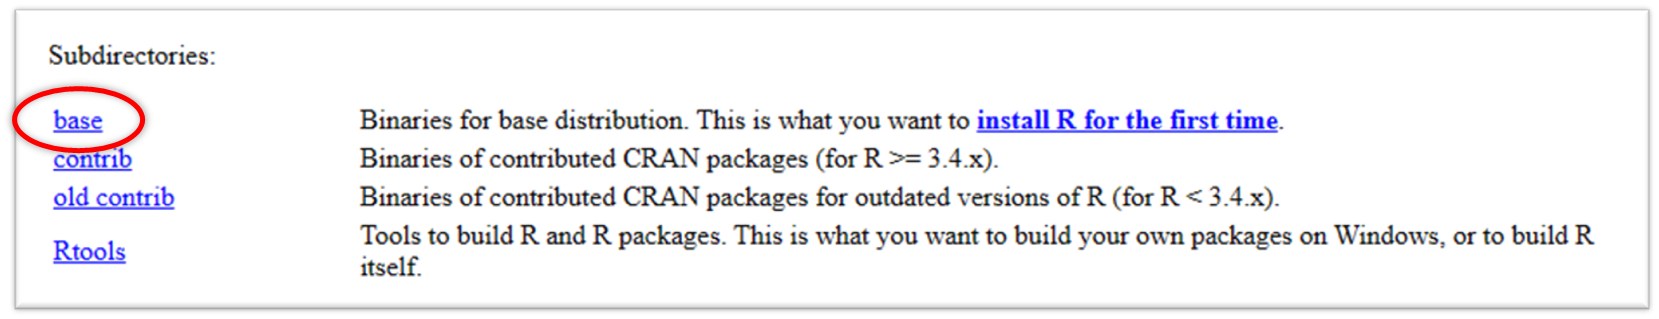
\includegraphics{images/clipboard-959933518.png}
  \end{center}
\item
  Na nova página, clique em `\emph{Download R x.x.x for Windows}', sendo
  `x.x.x' o número da versão que será baixada. No momento da elaboração
  deste tutorial, a versão mais recente do R é a 4.3.3.

  \begin{center}
  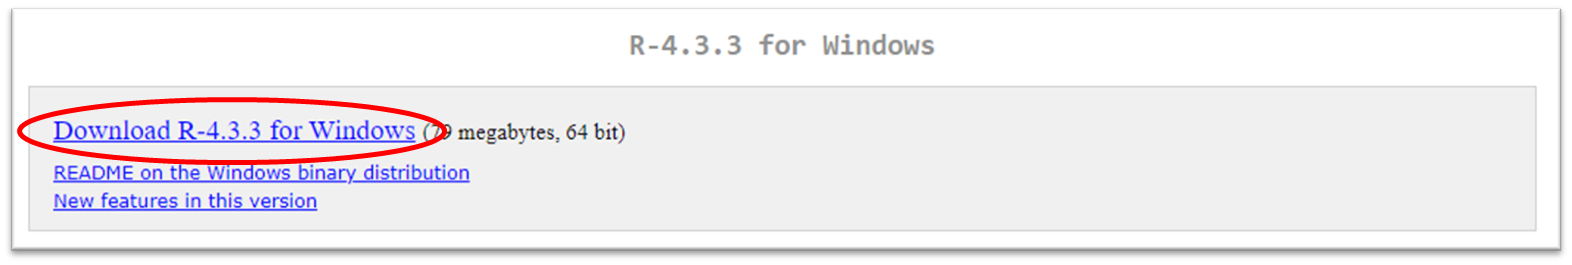
\includegraphics{images/clipboard-3581535596.png}
  \end{center}

  Se você tiver algum problema com o \emph{download}, tente escolher
  outro servidor no passo 2 -- por exemplo, um dos servidores da
  Universidade de São Paulo.
\end{enumerate}

\begin{tcolorbox}[enhanced jigsaw, opacityback=0, breakable, leftrule=.75mm, toprule=.15mm, colbacktitle=quarto-callout-note-color!10!white, toptitle=1mm, colback=white, left=2mm, title=\textcolor{quarto-callout-note-color}{\faInfo}\hspace{0.5em}{Encontrando o caminho!}, bottomtitle=1mm, titlerule=0mm, arc=.35mm, rightrule=.15mm, bottomrule=.15mm, opacitybacktitle=0.6, coltitle=black, colframe=quarto-callout-note-color-frame]

Abaixo, os passos 1-5 para realizar o \emph{donwload}.

\begin{center}
\includegraphics{images/instalacao_r.gif}
\end{center}

\end{tcolorbox}

\begin{enumerate}
\def\labelenumi{\arabic{enumi}.}
\setcounter{enumi}{5}
\item
  Você receberá um aviso, que varia conforme o navegador em uso, de que
  o arquivo está sendo baixado. Abaixo, um exemplo no Microsoft Edge:

  \begin{center}
  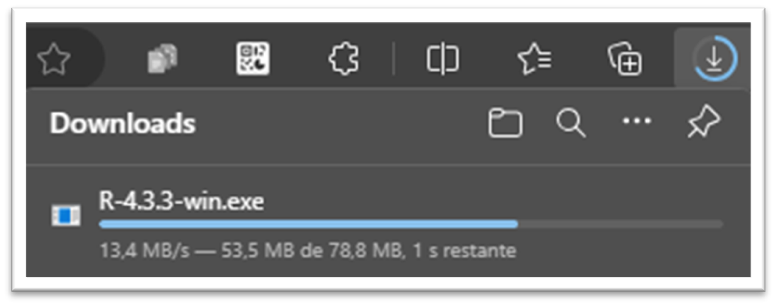
\includegraphics[width=3.96875in,height=\textheight]{images/clipboard-2313357345.png}
  \end{center}

  No Windows, o arquivo será armazenado na pasta `Downloads' do seu
  computador (ou na pasta que você previamente configurou como destino
  para os arquivos baixados).
\item
  Feito o download, clique duas vezes no arquivo baixado e siga as
  instruções para instalação. Na prática, basta clicar em `Avançar' até
  o fim.

  \begin{center}
  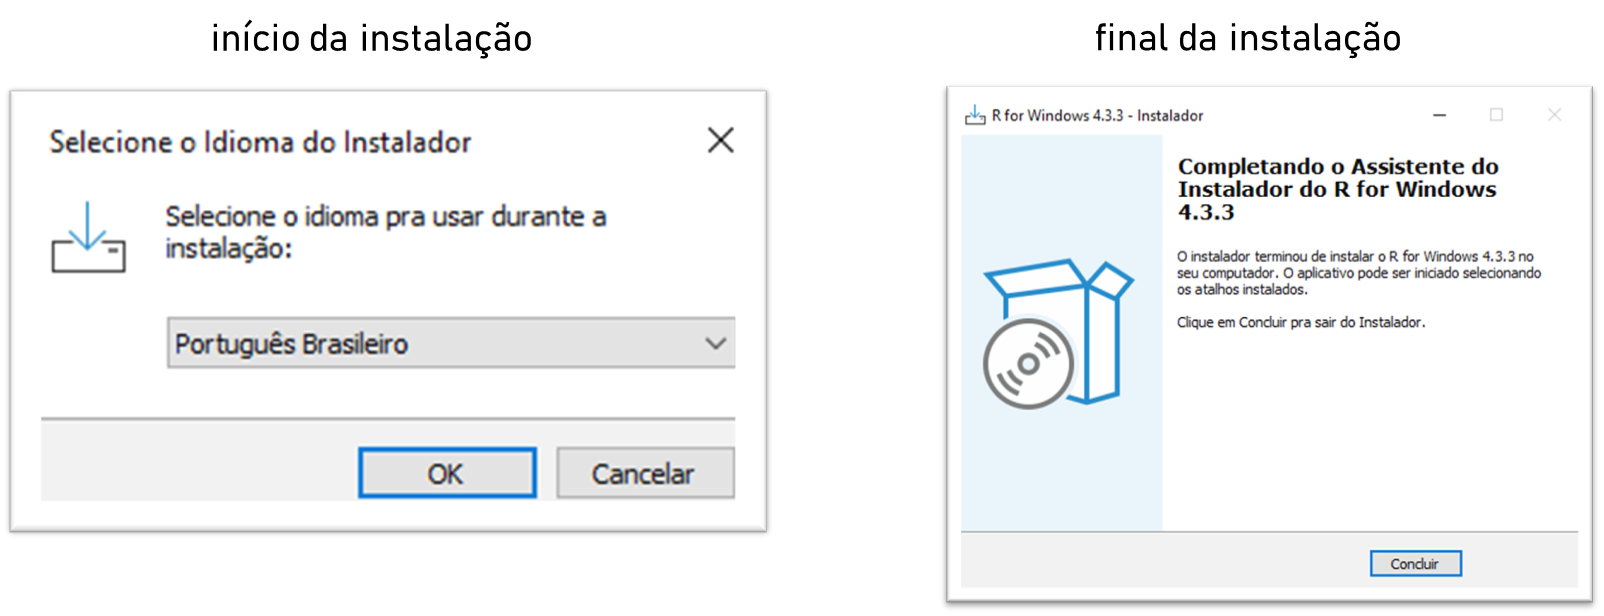
\includegraphics{images/clipboard-1694765597.png}
  \end{center}
\end{enumerate}

Após o final da instalação, você deverá ser capaz de encontrar e abrir
no seu computador o \textbf{R Graphical User Interface} ou, como
popularmente é conhecido, \textbf{RGui}. Ele estará na pasta em que você
destinou para instalação; no Windows, algo próximo de:

\texttt{C:\textbackslash{}ProgramData\textbackslash{}Microsoft\textbackslash{}Windows\textbackslash{}Start\ Menu\textbackslash{}Programs\textbackslash{}R}

\begin{center}
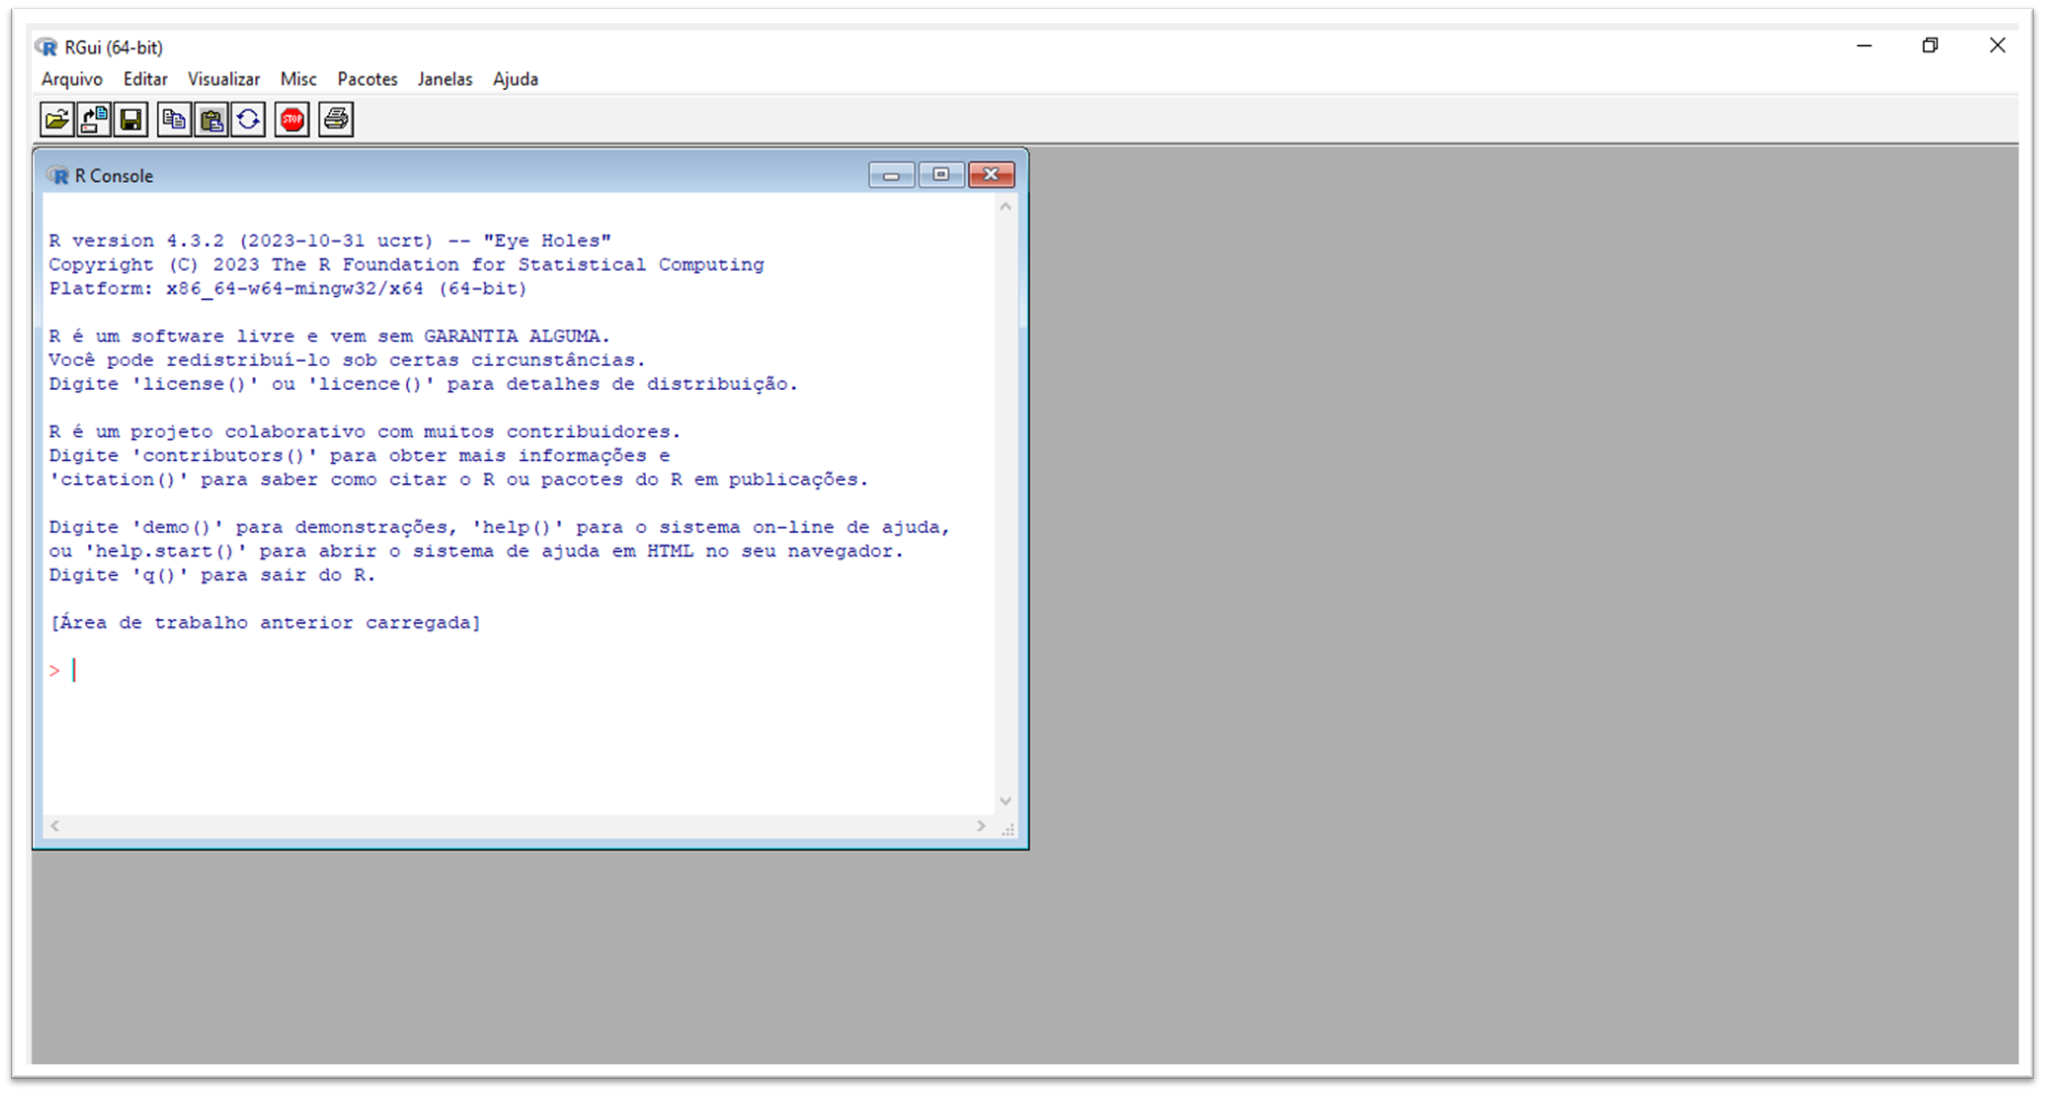
\includegraphics{images/clipboard-2094164095.png}
\end{center}

\section{Conhecendo o RGui}\label{conhecendo-o-rgui}

De forma geral, um GUI permite com que o usuário utilize a linguagem de
forma interativa através de botões e dispositivos visuais. Observe que,
na parte superior, temos oito botões principais, representados por
pequenas imagens.

\begin{center}
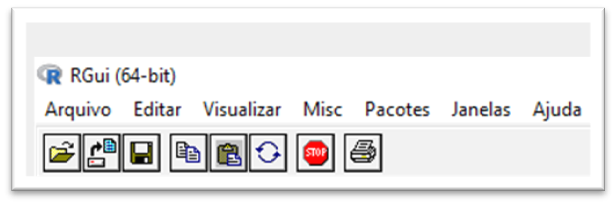
\includegraphics[width=3.125in,height=\textheight]{images/clipboard-3228534230.png}
\end{center}

Cada botão executa uma tarefa específica. Os três primeiros, da esquerda
para direita, são os mais relevantes:

\begin{itemize}
\item
  `Abrir script': permite com que você carregue, no Editor de Código, um
  arquivo que contém linhas de código (script). Arquivos desse tipo,
  cuja extensão é \texttt{.R}, serão os mais importantes da linguagem.
\item
  `Carregar área de trabalho': \emph{importa} objetos que foram salvos
  anteriormente em um arquivo do tipo \texttt{.RData}.
\item
  `Salvar área de trabalho': salva objetos criados em um arquivo do tipo
  \texttt{.RData}.
\end{itemize}

Os botões restantes, em ordem, executam as seguintes tarefas: `Copiar',
`Colar', `Copiar e colar', `Parar computação atual' e `Imprimir'. Nesse
momento, não se preocupe em saber o que significa \emph{importar} ou o
que é um arquivo do tipo \emph{.RData}.

Por outro lado, vamos procurar entender melhor o que são o
\textbf{Console} e o \textbf{Editor de Código}. O primeiro corresponde à
janela de nome \emph{R Console,} no canto esquerdo da sua tela. Este
último, por sua vez, não abre instantâneamente no momento em que você
acessa o RGui, mas podemos abrí-lo manualmente através de `Arquivo'
\textgreater{} `Novo script' -- ou, então, carregando um script já
existente através do botão `Abrir script', que vimos anteriormente.
Posicionando o Editor de Código ao lado do Console, teremos a seguinte
imagem:

\begin{center}
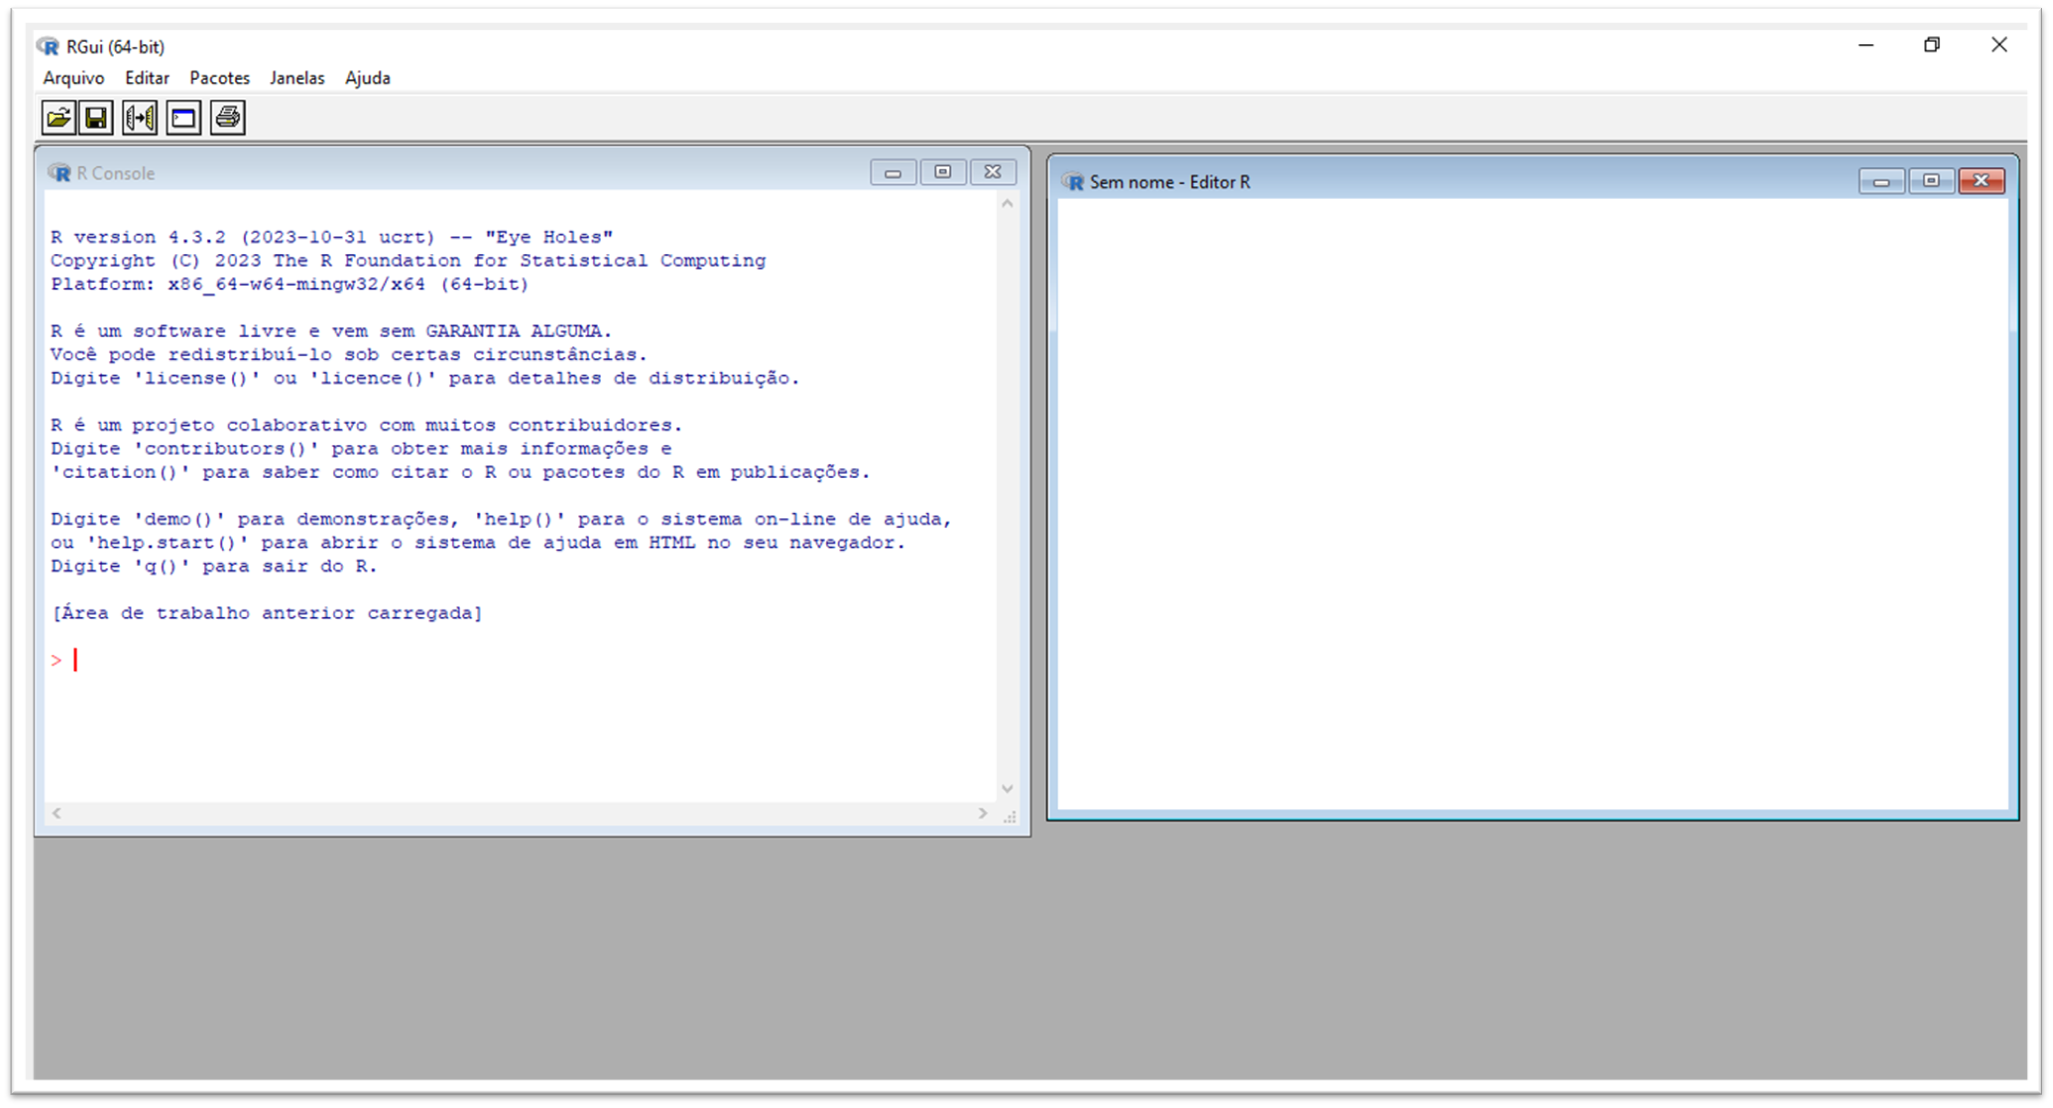
\includegraphics{images/clipboard-1401293353.png}
\end{center}

Por quê esses espaços terão relevância para nós?

\begin{itemize}
\item
  O Editor de Código é o local em que você escreve os comandos que
  deseja executar no R, além de comentários que busquem registrar o
  porquê de você ter escrito determinada parte do seu código. Na
  prática, um \emph{comentário} é uma linha que não será interpretada --
  e consequentemente executada -- como parte da linguagem. Para
  registrar um comentário, basta escrever o símbolo `\#' antes do que
  você deseja escrever naquela linha\footnote{Note que, se o seu
    comentário for longo demais, de tal forma que você queira quebrá-lo
    em duas ou mais linhas, será necessário novamente escrever `\#' na
    próxima linha}. Um ponto importante: o Editor permite com que
  salvemos o script que criamos em um arquivo do tipo \texttt{.R}.
  Lembre-se: esse é o principal tipo de arquivo da linguagem.
\item
  O Console, por sua vez, é o local em que a parte interpretável de
  código em R (ou seja, tudo exceto comentários) será
  \emph{efetivamente} executada e os respectivos resultados serão
  mostrados. É aqui que a mágica efetivamente ocorre! Você também pode
  executar partes do seu código diretamente no Console, porém os
  comandos não ficam salvos, são apenas temporários.
\end{itemize}

Simplificando: \textbf{o Editor é o espaço em que você realmente
escreverá os códigos em R}. Ele atua como rascunho do seu script,
permitindo com que você posteriormente salve o que foi escrito e,
consequentemente, volte a executar o mesmo código. Já \textbf{o Console
é o espaço em que o código é processado, retornando com o resultado dos
comandos que você escreveu}.

\textbf{Entretanto, não iremos utilizá-los através do RGui.} No capítulo
seguinte, instalaremos e conheceremos um pouco mais sobre outro
ambiente, bem mais completo, para se programar em R. \emph{``Meu Deus,
aprendi todos esses conceitos à toa?''}, você deve estar se perguntando.
Não! Muito do que aprendemos nessa seção voltará a aparecer no capítulo
seguinte.

\begin{tcolorbox}[enhanced jigsaw, opacityback=0, breakable, leftrule=.75mm, toprule=.15mm, colbacktitle=quarto-callout-tip-color!10!white, toptitle=1mm, colback=white, left=2mm, title=\textcolor{quarto-callout-tip-color}{\faLightbulb}\hspace{0.5em}{Executando um simples código no RGui (Opcional)}, bottomtitle=1mm, titlerule=0mm, arc=.35mm, rightrule=.15mm, bottomrule=.15mm, opacitybacktitle=0.6, coltitle=black, colframe=quarto-callout-tip-color-frame]

Beleza, não tocaremos no RGui. Mas é interessante compreender que já é
possível executar -- ou \emph{rodar,} no jargão de programação -- algum
pedaço de código -- ou \emph{chunk} -- escrito em R. Para isso, basta
escrevê-lo após o símbolo de `maior que' (\textgreater) no Console.

Vamos entender com um rápido exemplo. No GIF abaixo, atribuimos à
variável de nome \texttt{x} o valor númerico \texttt{2}. Em seguida,
escrevemos o nome novamente para retornar seu valor. Fique tranquilo:
ainda iremos ver melhor o que significam termos como \emph{atribuir um
valor à determinada variável}. O objetivo deste \emph{box} foi apenas te
mostrar que já estamos aptos a programar em R!

\begin{center}
\includegraphics{images/rgui_exemplo.gif}
\end{center}

\end{tcolorbox}

\bookmarksetup{startatroot}

\chapter{Instalando o RStudio}\label{instalando-o-rstudio}

\textbf{Acontece que o RGui não é tão prático de se usar}. Pensando
nisso, a empresa \href{https://posit.co/}{Posit} criou um Ambiente de
Desenvolvimento Integrado (\emph{Integrated Development Environment},
IDE) chamado \textbf{RStudio}. Em nosso contexto, tanto GUI quanto IDE
são ferramentas que permitem a utilização da linguagem. A diferença é
que a IDE tem atributos com a finalidade de facilitar o desenvolvimento
dos códigos. Grosso modo, toda IDE é uma GUI mas o inverso não é
verdadeiro (nem toda GUI é uma IDE).

Em resumo: \textbf{é muito mais fácil utilizar o R através do RStudio e,
por este motivo, vamos baixá-lo na sua versão gratuita} (que já é
suficiente para os cursos que serão ministrados no Instituto).

\section{Três passos}\label{truxeas-passos}

Para instalar o RStudio no Windows, novamente iremos seguir alguns
passos -- nesse caso, apenas 3:

\begin{enumerate}
\def\labelenumi{\arabic{enumi}.}
\item
  Acesse a página de downloads da RStudio:
  \url{https://posit.co/download/rstudio-desktop/\#download}. Se você
  tiver acesso de administrador, basta clicar em \emph{`Download RStudio
  Desktop for Windows'}.

  \begin{center}
  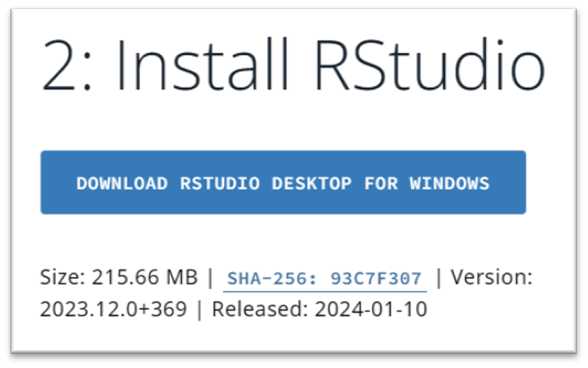
\includegraphics[width=3.32292in,height=\textheight]{images/clipboard-2426047081.png}
  \end{center}
\item
  De forma análoga ao \emph{download} do R, você receberá um aviso de
  que o arquivo está sendo baixado (na sua pasta de `Downloads' ou
  similar).

  \begin{center}
  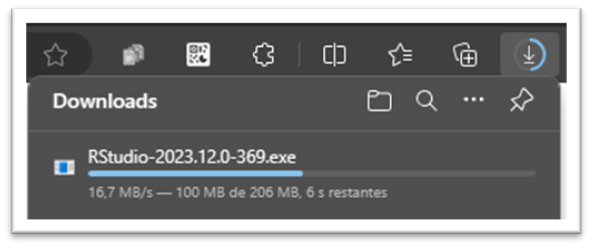
\includegraphics[width=3.85417in,height=\textheight]{images/clipboard-3795362132.png}
  \end{center}
\item
  Clique duas vezes no arquivo que você baixou e siga as instruções
  recomendadas de instalação, cuja tela inicial está na imagem abaixo.

  \begin{center}
  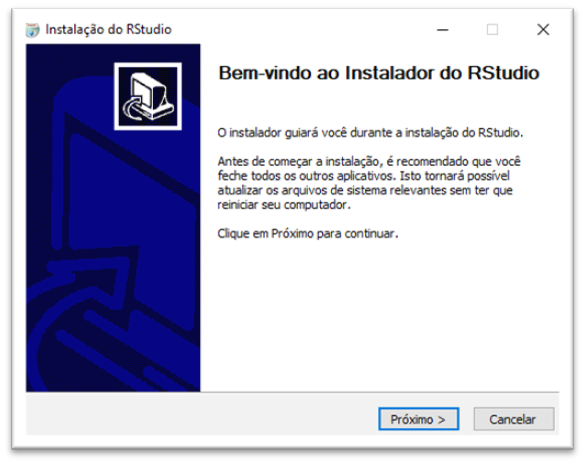
\includegraphics{images/clipboard-987499479.png}
  \end{center}
\end{enumerate}

Ao final da instalação, você deverá ser capaz de abrir o RStudio no seu
computador, resultando em algo similar à imagem abaixo. No Windows,
provavelmente você o encontrará no caminho:

\texttt{C:\textbackslash{}ProgramData\textbackslash{}Microsoft\textbackslash{}Windows\textbackslash{}Start\ Menu\textbackslash{}Programs\textbackslash{}RStudio}

\begin{center}
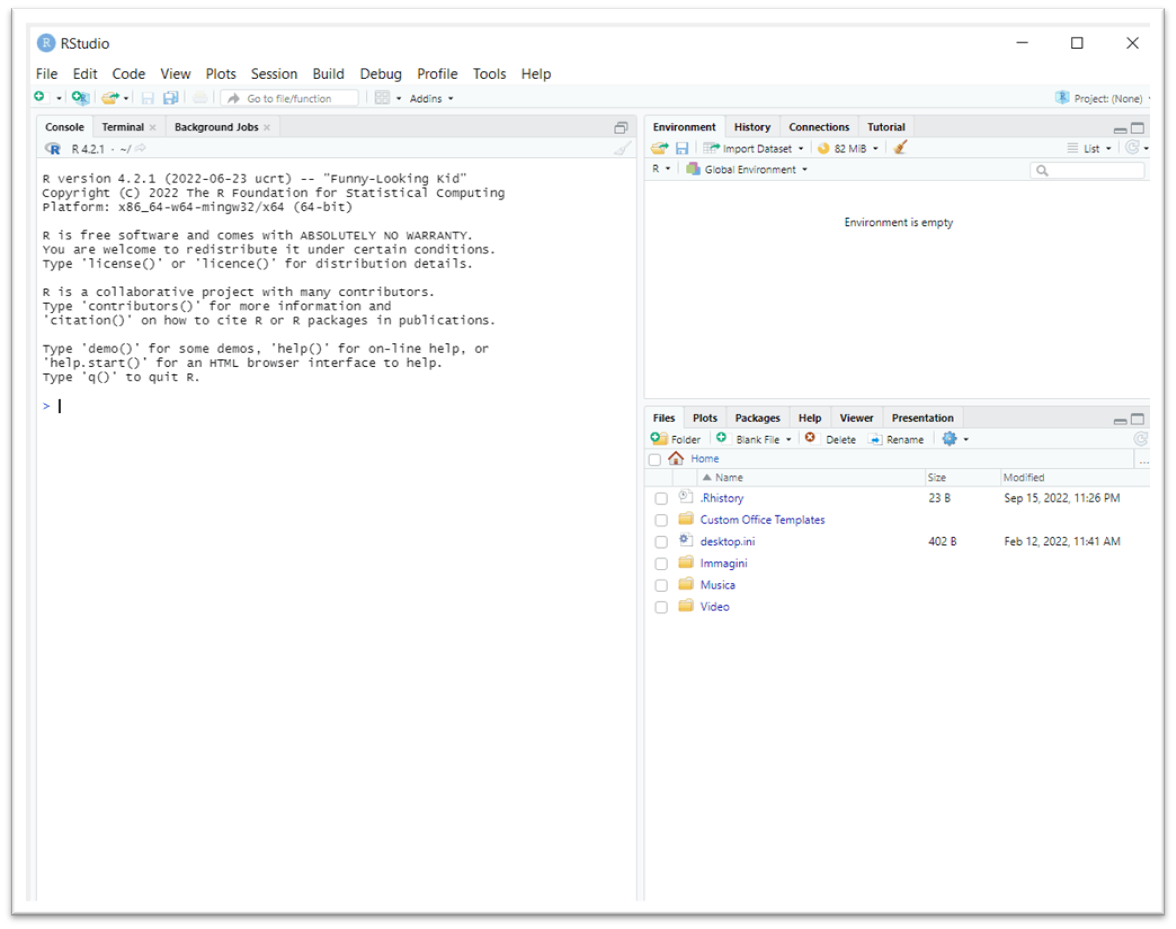
\includegraphics{images/clipboard-1128946571.png}
\end{center}

\textbf{Feito? Então estamos prontos para utilizar o R através do
RStudio!}

\section{Conhecendo o RStudio}\label{conhecendo-o-rstudio}

\begin{tcolorbox}[enhanced jigsaw, opacityback=0, breakable, leftrule=.75mm, toprule=.15mm, colbacktitle=quarto-callout-note-color!10!white, toptitle=1mm, colback=white, left=2mm, title=\textcolor{quarto-callout-note-color}{\faInfo}\hspace{0.5em}{Nota}, bottomtitle=1mm, titlerule=0mm, arc=.35mm, rightrule=.15mm, bottomrule=.15mm, opacitybacktitle=0.6, coltitle=black, colframe=quarto-callout-note-color-frame]

A seção 3.2 `Conhecendo o RStudio' é baseada na seção
\href{https://livro.curso-r.com/2-1-telas.html}{2.1 `Telas'} do livro
\emph{Ciência de Dados em R}, feito pelo Curso-R. De qualquer modo,
eventuais erros são inteiramente de nossa responsabilidade.

\end{tcolorbox}

O RStudio será o ambiente no qual iremos trabalhar com a linguagem. Por
essa razão, é \emph{muito} importante que você se sinta confortável com
o que verá no seu computador após abrí-lo. Nessa seção, iremos
compreender melhor o \emph{layout} do RStudio, além das utilidades que
ele nos proporciona ao longo do processo de escrita dos códigos.

Ao abrir o RStudio pela primeira vez (como na imagem anterior), você
verá inicialmente 3 quadrantes. Um deles, preenchendo a parte esquerda
da tela, já conhecemos: é o \textbf{Console}, que cumpre o mesmo papel
explicado no capítulo anterior. Ao mesmo tempo, o quadrante que mais
utilizaremos não aparece inicialmente: é o \textbf{Editor de Código},
outro velho conhecido que também possui a mesma atribuição anterior. Tal
como no caso do RGui, o Editor não abre automaticamente pois o RStudio
não é capaz de saber se o usuário tem o desejo de construir um código do
zero -- ou seja, criar um novo arquivo com extensão \emph{.R} -- ou
apenas dar continuidade à algum em que já estava trabalhando.

No fim das contas, teremos 4 quadrantes:

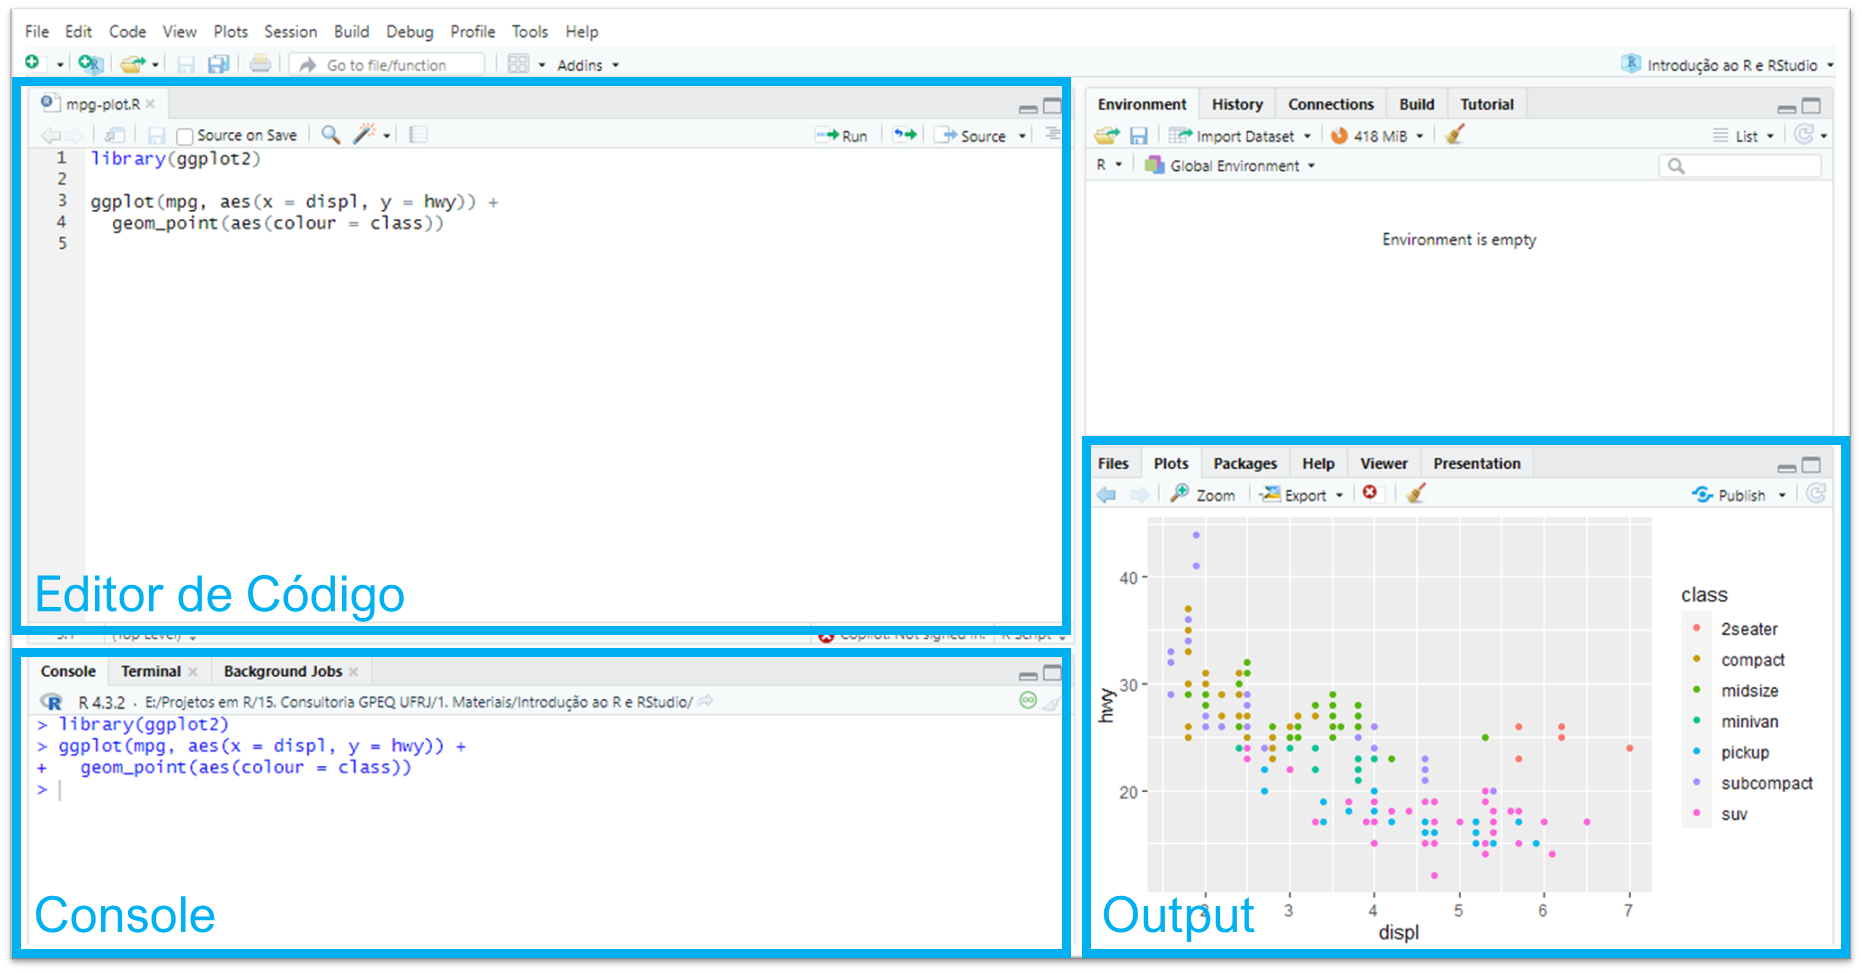
\includegraphics{images/clipboard-1486032127.png}

\begin{tcolorbox}[enhanced jigsaw, opacityback=0, colback=white, left=2mm, breakable, leftrule=.75mm, arc=.35mm, rightrule=.15mm, toprule=.15mm, bottomrule=.15mm, colframe=quarto-callout-note-color-frame]
\begin{minipage}[t]{5.5mm}
\textcolor{quarto-callout-note-color}{\faInfo}
\end{minipage}%
\begin{minipage}[t]{\textwidth - 5.5mm}

Por padrão, os quadrantes estarão dispostos na sua tela da forma como
mostramos na imagem acima, mas você pode organizá-los da forma que
preferir acessando a seção \emph{Pane Layout} da opção
\texttt{Global\ options...} no menu \texttt{Tools}.

\end{minipage}%
\end{tcolorbox}

É importante que você entenda que o Editor e o Console são os dois
principais quadrantes do RStudio. Passaremos a maior parte do tempo
neles. Como não custa nada, vamos relembrar suas respectivas serventias:

\begin{itemize}
\item
  \textbf{Editor de Código}: é local em que escreveremos/editaremos
  nossos códigos, salvando posteriormente em um arquivo do tipo
  \texttt{.R}. Conforme formos avançando, você acabará reparando que
  temos algumas melhorias em relação ao RGui:

  \begin{enumerate}
  \def\labelenumi{\arabic{enumi}.}
  \tightlist
  \item
    O RStudio colore algumas palavras e símbolos para \emph{facilitar} a
    leitura do código. Por exemplo, tudo o que for comentário será de
    uma determinada cor, assim como tudo que você escrever entre aspas
    -- considerado texto passível de ser executado como parte de um
    código -- será de outra.
  \item
    Outra funcionalidade interessante do Editor no RStudio é a
    capacidade de você poder buscar e substituir determinadas
    palavras/expressões que estejam presentes no código, poupando tempo
    e evitando erros caso o fizessemos de forma maunal; para tal, basta
    clicar no símbolo da lupa logo acima da primeira linha.
  \item
    Além disso, o RStudio possui o recurso de autocompletar partes de um
    código! Caso você esteja escrevendo o nome de um \emph{objeto} que
    ele consiga identificar, receberá automaticamente uma sugestão para
    completar a escrita, bastando apertar a tecla \texttt{Tab} para
    aceitá-la.
  \end{enumerate}
\item
  \textbf{Console}: é local em que o código é executado e recebemos as
  saídas. Nele, temos também o recurso de autocompletar nomes de
  objetos. Para \emph{limpar} o Console, isto é, excluir o registro do
  que já foi executado pelo R, basta clicar no símbolo de vassoura, no
  canto direito superior do quadrante, ou então utilizar o atalho
  \texttt{Ctrl\ +\ L}.
\end{itemize}

Os demais quadrantes do lado \emph{direito} contém painéis auxiliares. O
objetivo deles é facilitar pequenas tarefas que fazem parte tanto da
programação quanto da análise de dados como, por exemplo, olhar a
documentação de funções, analisar os objetos criados em uma sessão do R,
procurar e organizar os arquivos que compõem a nossa análise, armazenar
e analisar os gráficos criados e muito mais.

No quadrante \emph{superior}, temos

\begin{itemize}
\item
  \textbf{Environment}: painel com todos os objetos criados na sessão.
  Será bastante útil como referência para avaliar os objetos que criamos
  ou deixamos de criar com determinado comando.
\item
  \textbf{History}: painel com um histórico dos comandos rodados.
\end{itemize}

Já no quadrante \emph{inferior}, temos

\begin{itemize}
\item
  \textbf{Files}: mostra os arquivos no diretório de trabalho. Nele, é
  possível navegar entre as pastas do seu computador! Você pode, por
  exemplo, abrir um arquivo do tipo \texttt{.R} sem necessariamente ter
  que passar pela janela de busca do seu sistema operacional.
\item
  \textbf{Plots}: painel onde os gráficos serão apresentados, caso você
  crie um código que os produza.
\item
  \textbf{Packages}: apresenta todos os pacotes instalados e carregados.
\item
  \textbf{Help}: janela onde as documentações de funções serão
  apresentadas.
\item
  \textbf{Viewer}: painel onde relatórios e dashboards serão
  apresentados.
\end{itemize}

Além do Console e do Editor, dê atenção especial aos painéis
Environment, Help e Plots, nesta ordem.



\end{document}
